\section{Reactive walking pattern generator}

The balance control law of the robot takes as an input a velocity reference, and the system 
try to find footsteps such that the robot Center-Of-Mass is following as much as it can the velocity reference. 
In this PoC, two ways were tried to compute a reference velocity: visual servoing, and Euclidian distance between 
the object pose and the robot pose using a Motion Capture system. A more detailed description of the balance control 
law developed in the context of the French Research Project R-Blink is available in \cite{herdt:ar:2010}. 
A first experiment with this setup was realized in \cite{dune:iros:11}.

\begin{figure}
  \begin{center}
    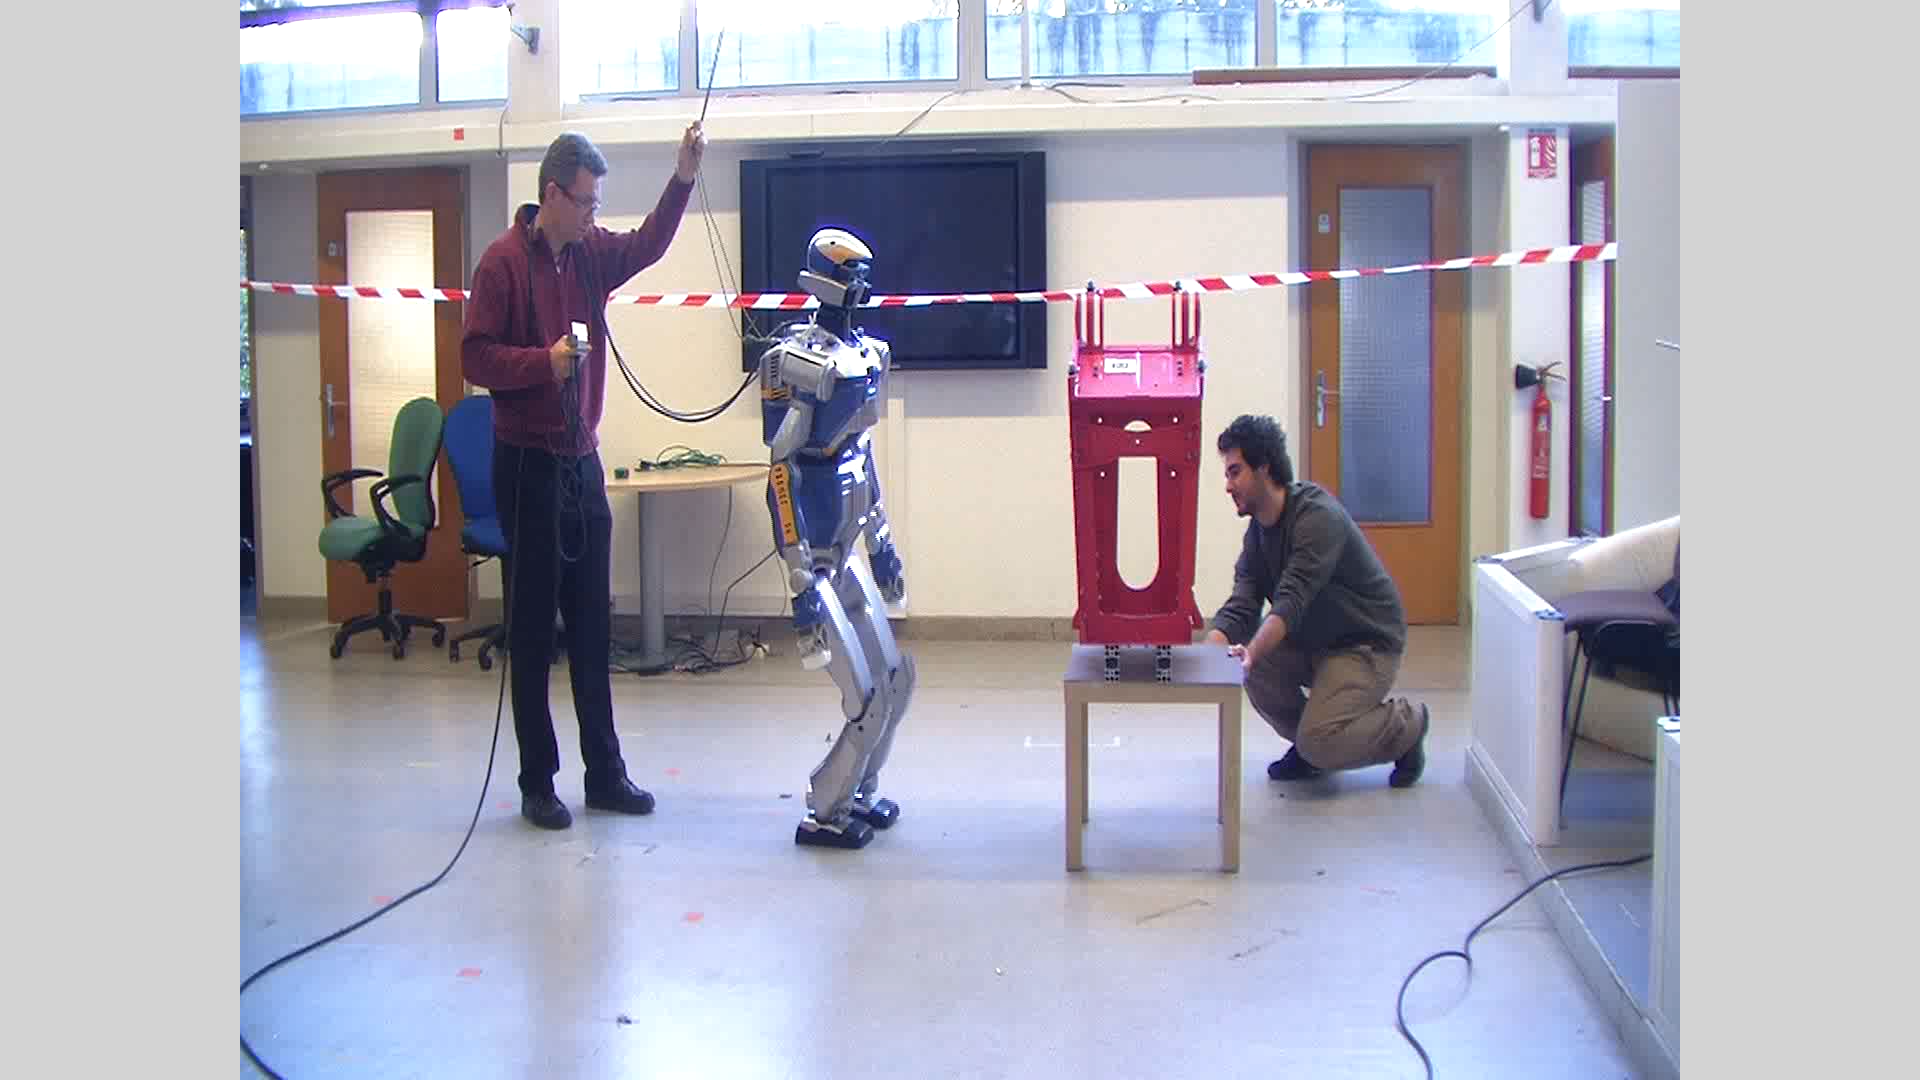
\includegraphics[clip=true, keepaspectratio, height=0.28\linewidth, trim={6.5cm 0cm 6.5cm 0cm}]{figures/engine_pylon.png}
    % trim={<left> <lower> <right> <upper>}
  \end{center}
  \caption{Robot tracking the engine pylon using a motion capture system}
  \label{fig:engine:pylon}
\end{figure}

In Fig.~\ref{fig:engine:pylon} the robot is able to follow the position of the engine pylon given by the motion capture system in the frontal plan.
This library was successfully used for the experiments described in \cite{dune:iros:11}. 
It was interesting to test it on a different HRP-2 to check the portability of the software.

Unfortunately if the ViSP library has been working quite well with the wooden mockup made by LAAS of the engine pylon, 
(as shown on the third section) it did failed with the 3D-print provided by Airbus. 
The main reason is the lack of sharp edge in the back of the pylon. 
We tried various strategies such as including a Kalman Filter, introducing knowledge in the tracker, 
but it turns out to be easier to use the Motion Capture System.
If this control law shows great promises, at this time it needed further improvement in the robustness part to be used in a repeatable setup. 
Our line of research was to improve the balance control by including the dynamic filter.
The dynamic filter has already been implemented and tested \cite{naveau:ichr:2014} and in Chap.~\ref{chap:nmpc} and the resolved momentum control is being implemented.


